\documentclass[12pt]{scrartcl}

\usepackage[english]{babel}
\usepackage[T1]{fontenc}
%\usepackage[noadjust]{cite}
\usepackage{url,color} % Citation numbers being automatically sorted and properly "compressed/ranged".
\usepackage{graphics,amsfonts}
\usepackage{epstopdf}
\usepackage[pdftex]{graphicx}
\usepackage[cmex10]{amsmath}
\usepackage{physics}
% Also, note that the amsmath package sets \interdisplaylinepenalty to 10000
% thus preventing page breaks from occurring within multiline equations. Use:
\interdisplaylinepenalty=2500
% after loading amsmath to restore such page breaks as IEEEtran.cls normally does.
\usepackage[utf8]{inputenc}
% Useful for displaying quotations
%\usepackage{csquotes}
% Compact lists
%\let\labelindent\relax
\usepackage{enumitem}
\usepackage{hhline}
\usepackage{wrapfig}
\usepackage{makecell}

\usepackage[bookmarksopen=false]{hyperref}
\usepackage{bookmark}
\usepackage[style=alphabetic,backend=biber]{biblatex}

%tikz figures
\usepackage{tikz}
\usetikzlibrary{automata,positioning,chains,shapes,arrows}
\usepackage{pgfplots}
\usetikzlibrary{plotmarks}
\newlength\fheight
\newlength\fwidth
\pgfplotsset{compat=newest}
\pgfplotsset{plot coordinates/math parser=false}

\usepackage{array}
% http://www.ctan.org/tex-archive/macros/latex/required/tools/
%\usepackage{mdwmath}
%\usepackage{mdwtab}
%mdwtab.sty	-- A complete ground-up rewrite of LaTeX's `tabular' and  `array' environments.  Has lots of advantages over
%		   the standard version, and over the version in `array.sty'.
% *** SUBFIGURE PACKAGES ***
%\usepackage[tight,footnotesize]{subfigure}
\usepackage{subfig}

\usepackage[top=1.5cm, bottom=2cm, right=1.6cm,left=1.6cm]{geometry}
\usepackage{indentfirst}

\usepackage{times}
% make sections titles smaller to save space
%\usepackage{sectsty}
%\sectionfont{\large}
% enable the use of 'compactitem', a smaller 'itemize'
%\usepackage{paralist}

% to split equations using dmath env
\usepackage{breqn}
% nice rules in tables
%\usepackage{booktabs}
\usepackage{tabu}
\usepackage{array}

% tabular positioning
\usepackage{dblfloatfix}
\usepackage{lipsum}

% for simil-Times New Roman
\usepackage{mathptmx}% http://ctan.org/pkg/mathptmx
% for inteline spacing
\linespread{1.5}



% bibliography
\addbibresource{tex/bibliography.bib}


\begin{document}
%\maketitle


\begin{titlepage}
	
\centering
{
\includegraphics[width=4cm]{img/logo_unipd}
\hspace{7cm}

\includegraphics[width=4cm]{img/logo_dei}
}

\vspace{2cm}
{\bfseries\Large\textit
	Wireless Communications\\
} 
{\bfseries\Huge
	Simulation of Multipath Fading Channels\\
}
\vspace{1cm}
{\large
	\textbf{Author:}
	
	\normalsize
	\begin{tabular}{ll}
		Mattia Lecci 	& {\footnotesize\textit{(1153428)}} \\ 
	\end{tabular} 
} 
\vfill

% total: min 5, max 15 pages
\begin{abstract}	% max 10 lines
{\Large\textbf{Abstract}}
\vspace{0.5cm}

Throughout the years, many wireless channel simulators have been proposed with different performance objectives. In this project I will implement 8 of them, explaining how they work, the differences from one another and, finally, testing statistical and computation performance, comparing all of them in order to find their strengths and weaknesses.

As expected, there is no single winner, but just two of them will show appreciable characteristics in separate performance indexes. You will see how the best performer will have below average statistical properties and how, maybe surprisingly, the original Clarke's model will actually yield the best overall statistical performance with comparable computational performance to more modern solutions

\end{abstract}

\end{titlepage}
\newpage
\section{Introduction} % max 1 page
\label{sec:introduction}

The report is structured as follow: in Section \ref{sec:technical_approach} I will present the techninical aspects of the project, starting from Subsection \ref{subsec:objectives} which delineates the main objectives, the in Subsection \ref{subsec:math_models} the mathematical models of all the implemented simulators will be carefully described and in Subsection \ref{subsec:scenario} an idea of the code structure will be presented. Finally, in Subsection \ref{subsec:complications} I will briefly talk about a few complications encountered while completing this project. In Section \ref{sec:results}, then, the results will be presented and lastly in Section \ref{sec:conclusions} the conclusions will be drawn.
\newpage
\section{Technical Approach}	% no limits given
\label{sec:technical_approach}



\subsection{Objectives} % max 5 lines
\label{sec:objectives}


\subsection{Scenario} % max 20 lines
\label{subsec:scenario}


\subsection{Mathematical models used} % no limits given
\label{subsec:math_models}

Almost all of the reference papers start by introducing the ideal statistical properties that a Rayleigh channel should have, obtained for the classical model of such channel. This model is presented in \cite{clarke} and it is often referred to as \textbf{Clarke}'s 2D isotropic (both scattering and antenna gain) Rayleigh fading model, given by%
%
\begin{equation}
X(t) = \frac{1}{\sqrt{N}} \sum_{n=1}^{N} e^{j(2\pi f_d \cos \alpha_n t + \phi_n)}
\end{equation}%
%
where N is the number of propagation paths, $f_d$ is the maximum Doppler frequency, $\alpha_n$ is the angle of arrival of the $n$-th ray and $\phi_n$ its initial phase. Both $\alpha_n$ and $\phi_n$ are uniformly distributed in $(-\pi,\pi]$ for all $n$ and they are mutually independent, for a total of $2 \times N$ random variables. Since in general a huge number of rays reaches the receiver at the same time, the \textit{Central Limit Theorem} (\textit{CLT}) justifies the approximation of the channel to a Complex Normal ($\mathcal{CN}$) distribution. To be honest, the independence of real and imaginary part (which is implied in the definition of \textit{Complex Normal} distribution) is not trivial, but it will not be further clarified here. From this, we know that the magnitude of a Complex Normal random variable yields a Rayleigh distributed one (since it's equivalent to the euclidean norm of a 2D Gaussian random vector) and, by the symmetry of the distribution, the phase is uniformly distributed in $(-\pi,\pi]$. In formulas,%
%
\begin{subequations} \label{eqs:pdfs}
\begin{align}
	f_{|X|}(x) = 2x \ e^{-x^2}, \quad x \geq 0\\
	f_{\theta}(x) = \frac{1}{2\pi}, \quad x \in (-\pi,\pi]
\end{align}
\end{subequations}%
%
As $N$ tends to infinity, defining $X(t) = X_c(t) + jX_s(t)$ it is possible to prove the following correlations:%
%
\begin{subequations}
	\label{eqs:correlations}
\begin{align}
&R_{X_cX_c}(\tau) = E[X_c(t)X_c(t-\tau)] = \frac{1}{2} J_0(2\pi f_d\tau)\\
&R_{X_sX_s}(\tau) = \frac{1}{2} J_0(2\pi f_d\tau)\\
&R_{X_cX_s}(\tau) = R_{X_sX_c}(\tau) = 0\\
&R_X(\tau) = E[X(t) X^*(t-\tau)] = J_0(2\pi f_d \tau)\\
&R_{|X|^2}(\tau) = 1 + J_0^2(2\pi f_d \tau)
\end{align}
\end{subequations}%
%
Where $J_0(x)$ is the zero-order Bessel function of the first kind, defined as%
%
\begin{equation}
J_0(x) = \frac{1}{\pi} \int_0^\pi \cos( x \ \cos\theta) \dd{\theta}
\end{equation}%
%
As you can see, all of these correlations are obtained from a \textit{Wide Sense Stationary} (\textit{WSS}) process, since they only depend on the variable $\tau$.\\
Another two very interesting properties which can be extracted from \textit{Clarke}'s model are called \textit{Level Crossing Rate} (\textit{LCR}) and \textit{Average Fade Duration} (\textit{AFD}). They both characterize what happen at certain thresholds for the wireless channel and it's generally a higher order behavior: while \textit{LCR} determines the rate at which the envelope crosses a thresholds with positive slope, \textit{AFD} indicates for how long the channel will stay below the given threshold in average. They are clearly important parameters to consider when designing a wireless system, in particular when designing an appropriate channel coding. Ideally, their formulas are respectively:%
%
\begin{align}
L_{|X|}(\lambda) &= \sqrt{2\pi} f_d \lambda e^{-\lambda^2} \label{eq:LCR} \\
T_{|X|}(\lambda) &= \frac{e^{\lambda^2} - 1}{\sqrt{2\pi} f_d \lambda} \label{eq:AFD}
\end{align}%
%
where $\lambda$ is the normalized fading envelope threshold defined as $\lambda = |X_{thr}|/|X_{rms}|$. Since we are dealing with unit power simulations, then, $\lambda$ is simply equal to the threshold itself.

% ----------------------------------------------------------------------
% Jakes
%-----------------------------------------------------------------------
Since \textit{Clarke}'s model deals with multiple complex sinusoids and random variables, which are both computationally expansive to calculate, \textbf{Jakes} proposed in \cite{jakes} its well known simplification of such model, which basically became a standard for wireless channel simulation for over 20 years. In order to cut down on computational complexity he makes some assumptions: instead of being random variables, he forces $\alpha_n = \frac{2\pi n}{N}$ and correlates $\phi_n$ in quadruplets to obtain the following simplified model:%
%
\begin{subequations}
\begin{align}\label{eq:jakes_xc}
X_c(t) &= \sqrt{\frac{2}{N}} \left[ \cos(2\pi f_d t) + \sum_{n=1}^{M} 2\cos \left( \frac{\pi n}{M} \right) \cos( 2\pi f_d \cos \alpha_n \ t) \right]\\
\label{eq:jakes_xs}
X_s(t) &= \sqrt{\frac{2}{N}} \left[ \cos(2\pi f_d t) + \sum_{n=1}^{M} 2\sin \left( \frac{\pi n}{M} \right) \cos( 2\pi f_d \cos \alpha_n \ t) \right]
\end{align}
\end{subequations}%
%
You can see that the model is now fully deterministic and there are about a quarter of the oscillators of the corresponding Clarke's model. In fact, by defining $N = 4M+2$, there are only $M+1$ low frequency oscillators needed. Note that the directions with maximum Doppler spread are forcefully kept.

% ----------------------------------------------------------------------
% Pop Beaulieu
%-----------------------------------------------------------------------
This, though, comes at a price: \textbf{Pop} and \textbf{Beaulieu} state in \cite{A1} that Jakes' simulator is not even stationary and yields poor higher order statistics. To overcome this phenomena, a simple modification is proposed: the addition of an initial random phase to the low frequency oscillators. From Eqs.~\ref{eq:jakes_xc},\ref{eq:jakes_xs} the oscillator terms become: $\cos(2\pi f_d t + \phi_0)$ and $\cos( 2\pi f_d \cos \alpha_n \ t + \phi_n)$, where $\phi_n$ ($n=0,...,M$) are mutually independent uniform random variables in $(-\pi,\pi]$.\\
Now, a small modification that I did with respect to the original paper is the addition of the multichannel support. This may be useful in different interesting scenarios: multiple independent channels are usually used to model frequency selective fading and MIMO systems. I, instead, used this feature to estimate all the statistics of the simulators without relying on any kind of ergodicity. For the case of \textit{Pop-Beaulieu}'s simulator, this addition is very simple: calling $X_k(t)$ the $k$-th channel ($k=0,1,...,K-1$), we just need to generate $K \times(M+1)$ random variables $\phi_{k,n}$.

% ----------------------------------------------------------------------
% Zheng Xiao 2002
%-----------------------------------------------------------------------
In 2002, \textbf{Zheng} and \textbf{Xiao} \cite{C2} propose a novel simulator directly considering the multichannel scenario. The following formulas are given:%
%
\begin{subequations}
\begin{align}
X_{k,c}(t) &= \frac{1}{\sqrt{M}} \sum_{n=1}^{M} \cos \left( 2\pi f_d t \cos \left( \frac{2\pi n - \pi + \theta_k}{4M}\right) + \phi_{n,k}^{(c)} \right)\\
X_{k,s}(t) &= \frac{1}{\sqrt{M}} \sum_{n=1}^{M} \cos \left( 2\pi f_d t \sin \left( \frac{2\pi n - \pi + \theta_k}{4M}\right) + \phi_{n,k}^{(s)} \right)
\end{align}
\end{subequations}%
%
where $\theta_k, \ \phi_{n,k}^{(c)}$ and $\phi_{n,k}^{(s)}$ are mutually independent random variables uniformly distributed in $(-\pi,\pi]$, for a total of $K \times (2M+1)$ random variables. This ensures that all the channels have the same statistical properties while being uncorrelated. Note that with respect to the \textit{Pop-Beaulieu} model it adds randomness on the angle of arrival $\alpha_n$ and uncorrelates the initial phases of real and imaginary components, while not retaining the angles with maximum Doppler spread, having then $N=4M$. This means more than double the quantity of random variables required to perform the simulation, but a similar number of oscillators.

% ----------------------------------------------------------------------
% Li Huang
%-----------------------------------------------------------------------
Later in 2002, \textbf{Li} and \textbf{Huang} \cite{C1} proposed another multichannel simulator. Instead of randomizing the directions of arrival, they follow a deterministic approach, similar to \textit{Jakes}'. Defining $\alpha_{n,k} = \frac{2\pi n}{N} + \frac{2 \pi k}{NK} + \alpha_{0,0}$ for $n = 0,...,M-1$ and $k=0,...,K-1$, the formulas for the $k$-th ray are:%
%
\begin{subequations}
\begin{align}
X_{k,c}(t) &= \frac{1}{\sqrt{M}} \sum_{n=0}^{M-1} \cos \qty( 2\pi f_d t \cos \alpha_{n,k} + \phi_{n,k}^{(c)} )\\
X_{k,s}(t) &= \frac{1}{\sqrt{M}} \sum_{n=0}^{M-1} \sin \qty( 2\pi f_d t \sin \alpha_{n,k} + \phi_{n,k}^{(s)} )
\end{align}
\end{subequations}%
%
as usual $\phi_{n,k}^{(c)}$ and $\phi_{n,k}^{(s)}$ are mutually independent random variables uniformly distributed in $(-\pi,\pi]$, for a total of $2\times M \times K$ random variables. It is highlighted the fact that any combination of sine and cosine functions will not affect the actual statistics of the channels. The choice $\alpha_{0,0}$ is suggested by the authors to be in $\qty(0,\frac{2\pi}{NK}) \setminus \qty{\frac{\pi}{NK}}$. In the end I decided to use their same initial angle, meaning $\alpha_{0,0} = \frac{\pi}{2NK}$. The paper then also tries to reduce the high cost of calculating trigonometric functions by proposing different approximations and comparing then the results. I decided, though, to not implement this further in-depth analysis.

% ----------------------------------------------------------------------
% Zheng Xiao 2003
%-----------------------------------------------------------------------
Going on to 2003, \textbf{Zheng} and \textbf{Xiao} \cite{A2} further enhance their simulator by adding a random gain to each oscillator:%
%
\begin{subequations}
\begin{align}
X_{k,c}(t) &= \frac{1}{\sqrt{M}} \sum_{n=1}^{M} \cos(\psi_{n,k})\cos \left( 2\pi f_d t \cos \left( \frac{2\pi n - \pi + \theta_k}{4M}\right) + \phi_k \right)\\
X_{k,s}(t) &= \frac{1}{\sqrt{M}} \sum_{n=1}^{M} \sin(\psi_{n,k})\cos \left( 2\pi f_d t \cos \left( \frac{2\pi n - \pi + \theta_k}{4M}\right) + \phi_k \right)
\end{align}
\end{subequations}%
%
Note that the randomization of the angle of arrival is just the same as their 2002 paper but there are a couple of differences: the initial phase of the oscillators is now constant for all of the oscillators of the same channel (and equal for real and imaginary parts, similarly to the \textit{Pop-Beaulieu} model), whereas the difference between oscillators of the same channel is given by the random amplitude, which, even though it's different, it is correlated between real and imaginary components ($\psi_{n,k}$ is the same for both of them). A total of $K \times (M+2)$ random variables is needed.

% ----------------------------------------------------------------------
% Xiao Zheng Beaulieu
%-----------------------------------------------------------------------
In 2006, the most recent paper about \textit{Sum of Sinusoids} simulator that I considered was written by \textbf{Xiao}, \textbf{Zheng} and \textbf{Beaulieu} \cite{B1}. Once again, the simulator is a \textit{SoS} and introduces slight differences with respect to the others%
%
\begin{subequations}
	\begin{align}
	X_{k,c}(t) &= \frac{1}{\sqrt{M}} \sum_{n=1}^{M} \cos \left( 2\pi f_d t \cos \left( \frac{2\pi n  + \theta_{n,k}}{M}\right) + \phi_{n,k} \right)\\
	X_{k,s}(t) &= \frac{1}{\sqrt{M}} \sum_{n=1}^{M} \sin \left( 2\pi f_d t \cos \left( \frac{2\pi n  + \theta_{n,k}}{M}\right) + \phi_{n,k} \right)
	\end{align}
\end{subequations}%
%
The main differences with previous models are: no random amplitude for the oscillators is present, both $\theta$ and $\phi$ are independent between channels and oscillators (with a total number of $2 \times K \times M$ random variables required) although they are the same for real and imaginary components, the angle of arrival $\alpha_{n,k}$ has changed using only $M$ instead of $4M$ as the denominator. Similarly to the 2 previous papers from Zheng and Xiao, the angle of arrival is randomized but within sectors, in order to force a "more uniform" distribution, particularly for small values of $M$, with respect to the pure uniform distribution of the original Clarke's model.

% ----------------------------------------------------------------------
% Komninakis
%-----------------------------------------------------------------------
As the last one, I decided to keep the \textbf{Komninakis} simulator \cite{A3} since it's completely different from all the others, even though it's actually from 2003. In fact, while all the previous ones are based on the \textit{Sum of Sinusoids} method, this one works based on a \textit{filtering} method.%
%
\begin{figure}[h!]
	\centering
	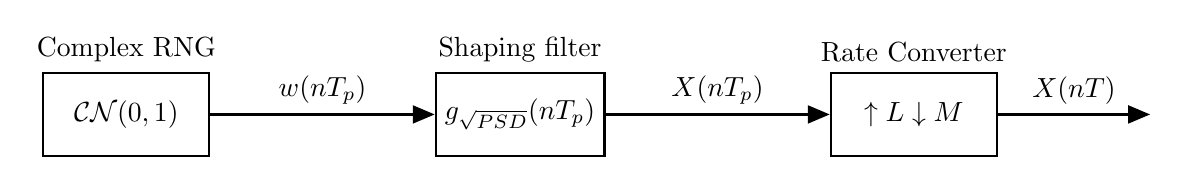
\begin{tikzpicture}[auto, thick, node distance=5cm, >=triangle 45]
% Definition of blocks:
\tikzset{%
	block/.style = {draw, thick, rectangle, minimum height = 3em,
		minimum width = 6em},
	input/.style = {coordinate}, % Input
	output/.style = {coordinate} % Output
}

% nodes
\draw node[block, name=gen, label={Complex RNG}] {$\mathcal{CN}(0,1)$};
\draw node[block, name=filt, right of=gen, label={Shaping filter}] {$g_{\sqrt{PSD}}(nT_p)$};
\draw node[block, name=interp, right of=filt, label={Rate Converter}] {$\uparrow L \downarrow M$};
\draw node[output, name=out, right of=interp, node distance=3cm] {};

% links
\draw[->] (gen) -- node[anchor=south]{$w(nT_p)$} (filt);
\draw[->] (filt) -- node[anchor=south]{$X(nT_p)$} (interp);
\draw[->] (interp) -- node[anchor=south]{$X(nT)$} (out);

\end{tikzpicture}
	\caption{Block diagram for \textit{Komninakis'} simulator}
\end{figure}

The basic idea is the following: starting from a white process $w(t)$ (which has constant \textit{Power Spectral Density}), in principle it is possible to obtain a stochastic process $X(t)$ with arbitrary PSD filtering it through an LTI system with frequency response $G_{\sqrt{PSD}}(f)$ since $\mathcal{P}_X(f) = \mathcal{P}_w |G_{\sqrt{PSD}}(f)|^2$, where the magnitude of the frequency response of the filter equals the square root of the desired PSD. In practice, though, it is not trivial to create a filter with arbitrary shape. In its paper, Komninakis proposes a way of approximating the magnitude of an IIR filter to a desired shape (in particular the classical PSD given by Clarke's model). There is one more problem to solve: particularly when modeling bit-level simulations, the sampling period $T$ may be much smaller than the \textit{coherence period} usually defined as $T_{coh}=\frac{1}{f_d}$. Equivalently, it means that the sampling frequency $F = \frac{1}{T} \gg f_d$, thus a very narrowband filter $G_{\sqrt{PSD}}$ would be required in order to correctly produce the desired output. It is widely known, though, that narrowband filters tend to require very high order which mean lots of calculations per sample to be done, very long transients and possible numerical instabilities given by the fact that poles have to be very close to the unit circle. This is definitely not the way to proceed. It is much wiser to filter at a much higher period $T_p$, computing only one or two filters with fixed values for the product $f_dT_p$ in order to balance order, stability and complexity, considering that an interpolation (or in general a rate conversion) will have to be done later. Note that the most correct way to perform the interpolation would be an up-sampling with zero padding followed by a low pass filter (either using low order IIR filter or a polyphase FIR filter). If the product $f_dT_p$ is small, though, it means that the channel will be slowly changing with respect to the chosen sampling period. This would allow us to use a simpler piecewise polynomial interpolation.\\
The big disadvantage of this simulator, then, becomes the high number of random variables needed. This depends, though, on the value of the product $f_dT_p$ for the reference shaping filter as well as the the actual product $f_dT$ needed. It, then, depends linearly on both the number of channels and length of the simulation required. One last thing to notice is that, if using a low pass filter for the interpolation, it has to be designed every time since any $f_dT$ product could be requested. For long simulations, though, a class instead of a function could be made so that filters would be designed only once and small pieces of channel could be computed one after the other in order to obtain simulations as long as necessary without incurring in huge memory requirements. Furthermore, adding the initial conditions for the filters as properties of the class, the obtained channel would really look like a single long continuous realization instead of multiple short disconnected ones.
\subsection{Complications found} % max 5 lines
\label{subsec:complications}

No major complications were found while doing this project. The only thing to be careful about was the different notation and normalization used in the various papers. Towards the end it has also been non trivial how to choose all of the numerous parameters for the simulation in order to properly highlight strengths and weaknesses of all the different models and how certain parameters affect the results.
\section{Results} % min 7 pages
\label{sec:results}

I'll present here statistical and performance results from all of the implemented simulators. The specific parameters have been chosen differently for almost every graph in order to emphasize its characteristics. For more details check out all the different \texttt{main} scripts that can be found in the folder \texttt{Code/}. Important parameters that I kept constant are $M=8$ (the number of oscillators for the simulators. Note that for \textit{Clarke}'s simulator $N=M$, while for all the other \textit{SOS} simulators $N \approx 4M$) and the interpolation method (for \textit{Komninakis'} simulator) chosen to be \texttt{pchip}. With this, MATLAB refers to a piecewise cubic polynomial interpolation with $C^1$ connections, instead of $C^2$ connection as for the more famous \texttt{spline}. A motivation for this choice will be given later on.

For all of the plots of the statistical results, a thick black line is firstly plotted with the ideal function, as described at the beginning of Section~\ref{subsec:math_models}.

%%%%%%%%%%%%%%%%%%%%%%%%%%%%%%%%%%%%%%%%%%%%%%%%%%%%%%%%%%%%%%%%%%%%%%%%%%%%%%%%%%%%%%%%%%%%%%%
%%%%%%%%% PDFs
%%%%%%%%%%%%%%%%%%%%%%%%%%%%%%%%%%%%%%%%%%%%%%%%%%%%%%%%%%%%%%%%%%%%%%%%%%%%%%%%%%%%%%%%%%%%%%%
\subsection{Probability Distribution Functions}

\begin{figure}
\hfill
\begin{minipage}{.49\linewidth}
	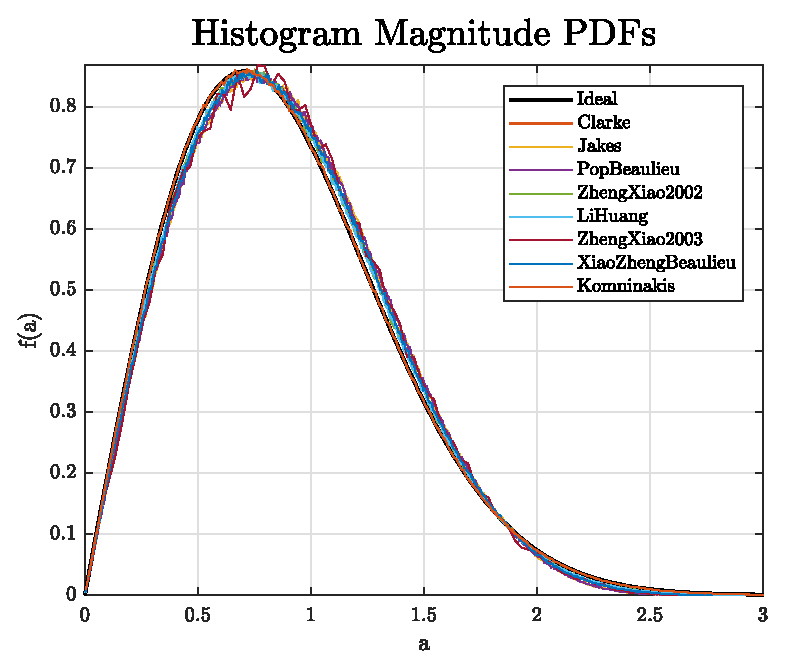
\includegraphics[width=\linewidth]{img/histMag.eps}
\end{minipage}
\hfill
\begin{minipage}{.49\linewidth}
	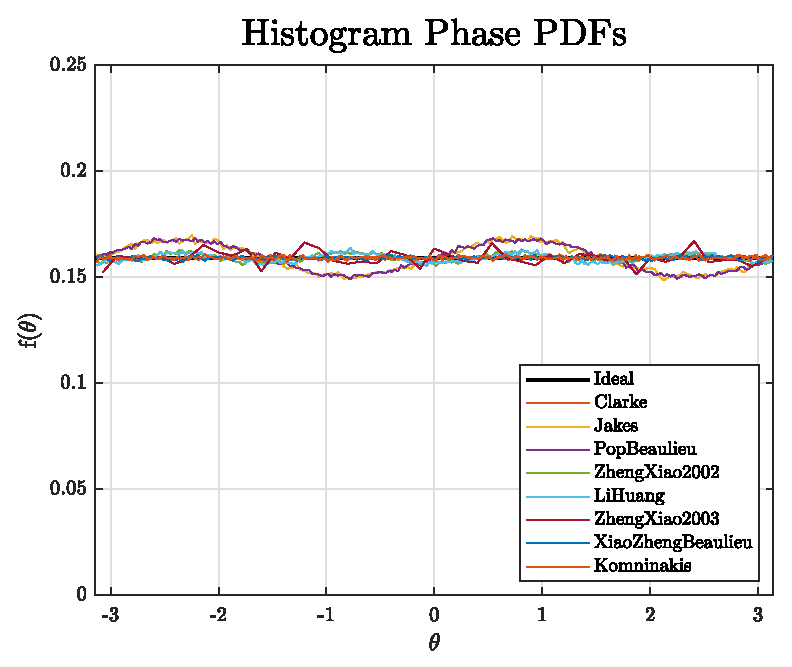
\includegraphics[width=\linewidth]{img/histPhase.eps}
\end{minipage}
\hfill

\caption{Histograms of Magnitudes and Phases of all the implemented simulators. Note the problem with \textit{ZhengXiao2003} and the pronounced wavy phase of \textit{Jakes'} and \textit{PopBeaulieu}'s simulators}
\label{fig:histograms}
\end{figure}

The first results presented are simple \textit{Probability Distribution Functions} (\textit{PDF}), for both magnitude and phase of the channels. Assuming stationarity, many independent channels of every simulators were created and MATLAB's \texttt{histogram} function was called on a specific samples across the channels. This was done to follow the probabilistic nature of the problem, avoiding the concept of ergodicity. One notable exception is \textit{Jakes'} simulator, which is fully deterministic, and thus its "\textit{PDF}" was calculated on the single realization. Another exception to this rule is \textit{ZhengXiao2003}: as it turns out, it is not really stationary. Calculating its PDF on the first sample, in fact, returned a very different result. To avoid this artifact, I created longer channels (about $T_{coh}$) and used the last sample instead. By doing this, though, I also had to provide less channels in order to not exceed memory limitations. The effect of this can be seen in Fig.~\ref{fig:histograms}, where \textit{ZhengXiao2003} has a rougher line.

Note, though, that all of the simulators approximate very accurately both \textit{PDF}s (Eqs.~\ref{eqs:pdfs}), with the exception of \textit{Jakes'} and \textit{PopBeaulieu}'s simulators which clearly have an oscillatory behavior instead of a constant one for what concerns the phase \textit{PDF}.

%%%%%%%%%%%%%%%%%%%%%%%%%%%%%%%%%%%%%%%%%%%%%%%%%%%%%%%%%%%%%%%%%%%%%%%%%%%%%%%%%%%%%%%%%%%%%%%
%%%%%%%%%%%% Correlations
%%%%%%%%%%%%%%%%%%%%%%%%%%%%%%%%%%%%%%%%%%%%%%%%%%%%%%%%%%%%%%%%%%%%%%%%%%%%%%%%%%%%%%%%%%%%%%%
\subsection{Correlations}

\begin{figure}
	\hfill
	\begin{minipage}{.49\linewidth}
		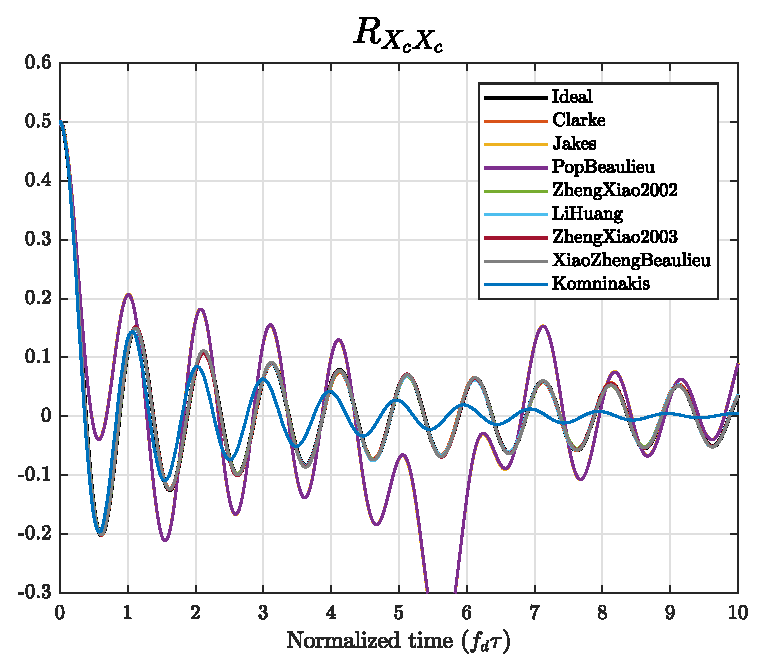
\includegraphics[width=\linewidth]{img/XcXc.eps}
	\end{minipage}
	\hfill
	\begin{minipage}{.49\linewidth}
		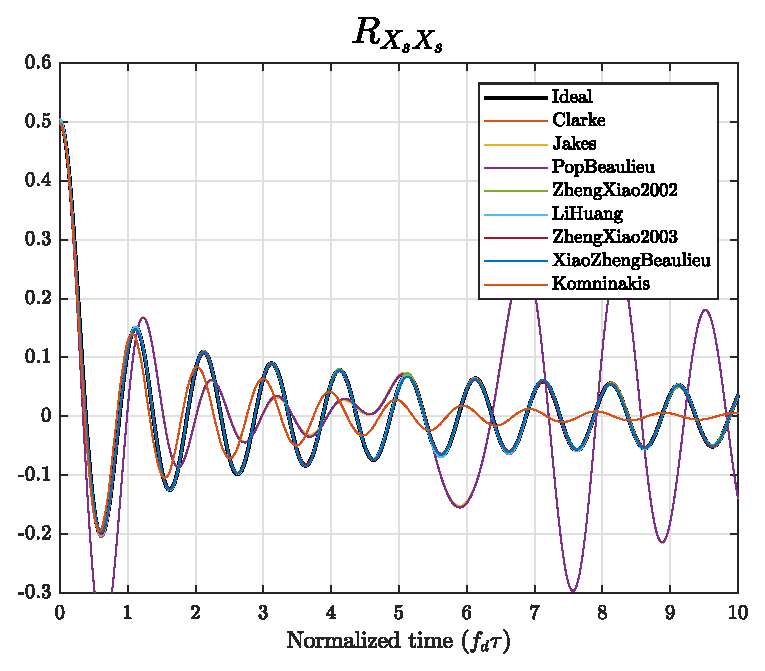
\includegraphics[width=\linewidth]{img/XsXs.eps}
	\end{minipage}
	\hfill
	
	\vspace{2mm}
	
	\hfill
	\begin{minipage}{.49\linewidth}
		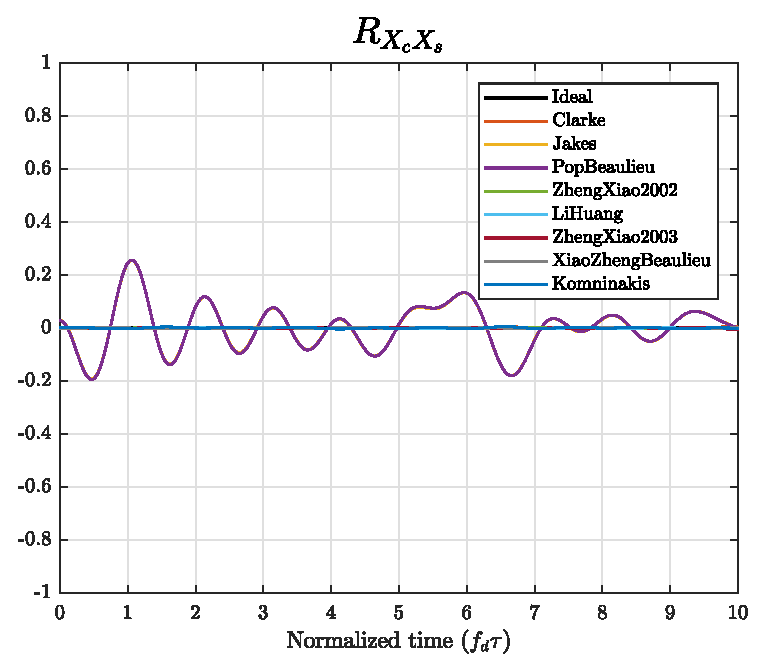
\includegraphics[width=\linewidth]{img/XcXs.eps}
	\end{minipage}
	\hfill
	\begin{minipage}{.49\linewidth}
		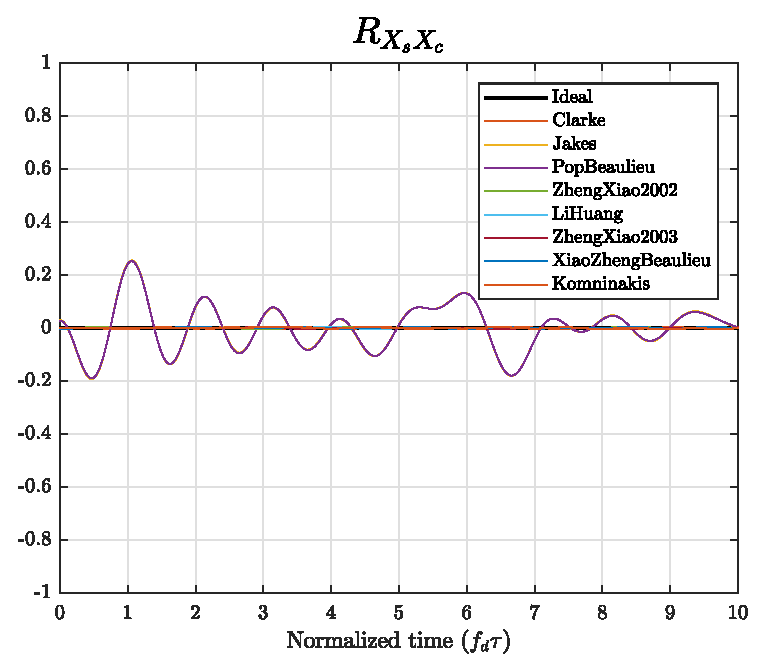
\includegraphics[width=\linewidth]{img/XsXc.eps}
	\end{minipage}
	\hfill
	
	\vspace{6mm}
	
	\hfill
	\begin{minipage}{.49\linewidth}
		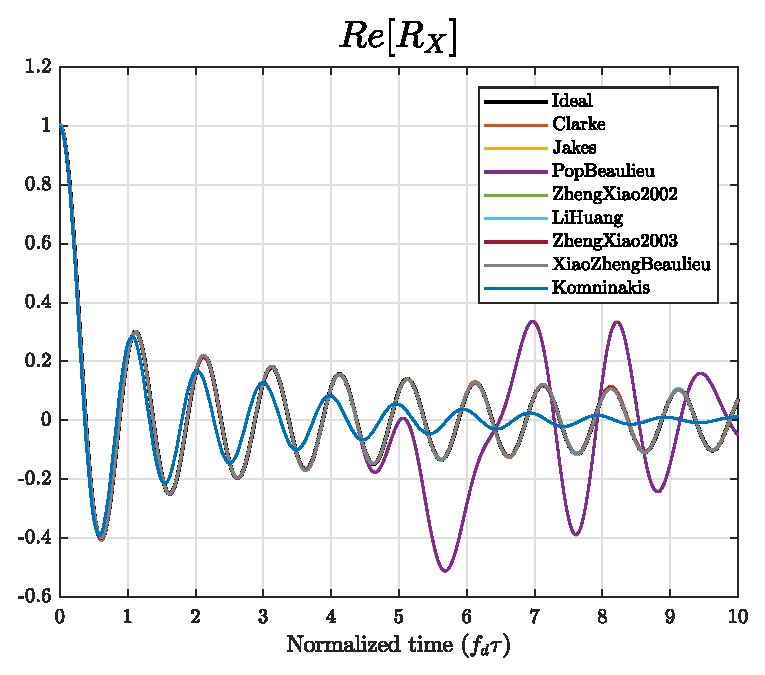
\includegraphics[width=\linewidth]{img/ReX.eps}
	\end{minipage}
	\hfill
	\begin{minipage}{.49\linewidth}
		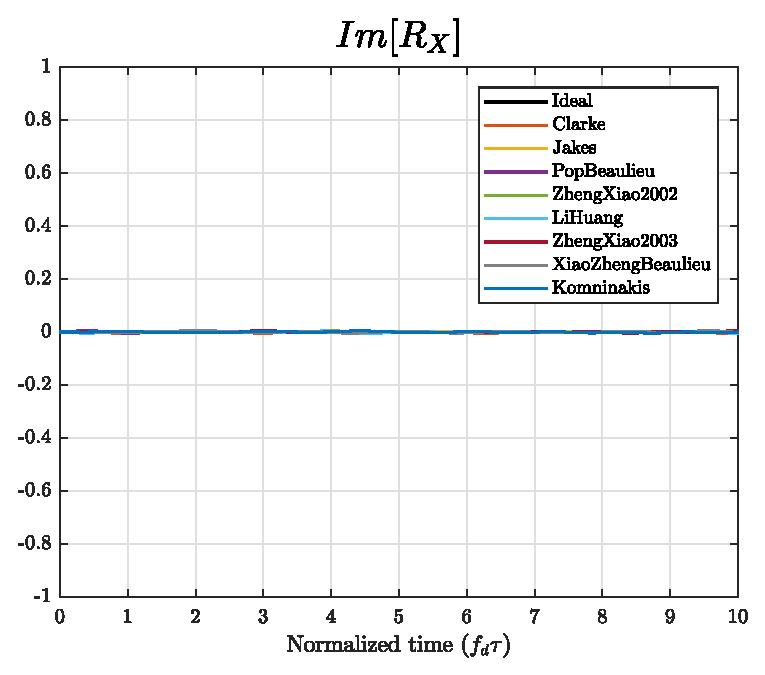
\includegraphics[width=\linewidth]{img/ImX.eps}
	\end{minipage}
	\hfill
	
	\caption{Cross correlations between real and imaginary components}
	\label{fig:xcorrs}
\end{figure}

Moving on to the correlations (Eqs.~\ref{eqs:correlations}, Figs.~\ref{fig:xcorrs}), it is clear that once again \textit{Jakes'} and \textit{PopBeaulieu}'s simulators cannot really match up with more modern solutions, resulting very early very imprecise especially when dealing with single real or imaginary components. For what concerns the correlation of the signal $X(t)$ as a whole, instead, they both tend to behave better, but still in the real part of $R_X$ they are both the first ones to significantly diverge from the ideal function.

\textit{Komninakis'} simulator is the other one that significantly diverges from the ideal case when non-zero functions are involved. Since its core idea is to design a filter that tries to mimic a given PSD (which I recall from \textit{Wiener–Khinchin theorem} is the \textit{Fourier Transform} of the autocorrelation function of the stochastic process), the reason why this happen should be a poor approximation of such filter. I also recall that I simply took the filter's coefficients from \cite{digital} without further investigations. It's clear from Fig.~\ref{fig:xcorrs}, though, that both the shape (quick ripple attenuation) and the Doppler frequency $f_d$ ("higher frequency" ripples) of this approximation are not really good. It should be possible, though, to improve this trading performance for accuracy.

All of the other simulators, instead, are almost indistinguishable from each other and from the ideal case, at least up to a normalized time $f_d\tau = 10$. I want to recall that this is obtained with only $8$ oscillators for all of these simulators! Note that also the original \textit{Clarke}'s simulator is indistinguishable from the ideal case with these few oscillators, and keep in mind that it's only a fourth of the equivalent number of oscillators simulated by the other designs. This is to empirically confirm the statement from \cite{B1} where \textit{Clarke}'s simulator is said to converge very quickly to the ideal case. This fact almost seems to suggest that \textit{Jakes'} simulator might not have been even needed in the first place!

\begin{wrapfigure}{R}{.45\linewidth}
	\centering
	\begin{minipage}{\linewidth}
		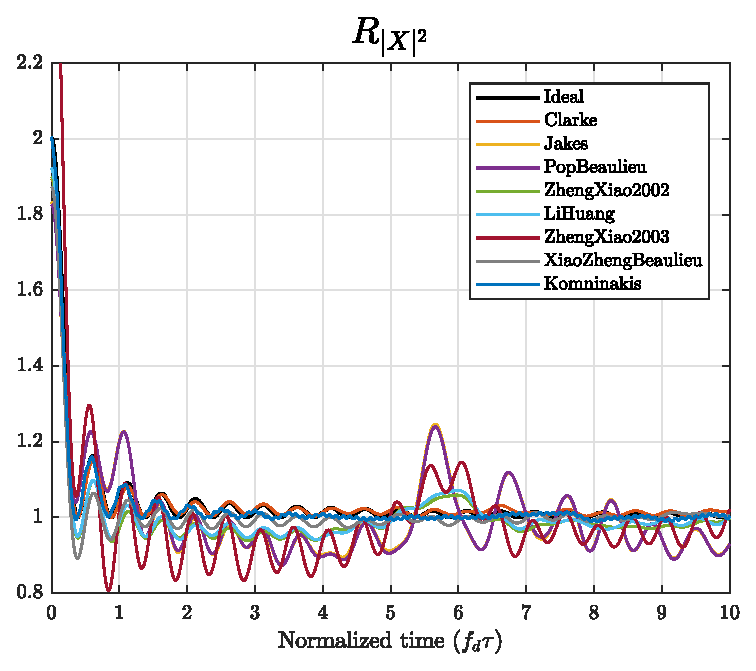
\includegraphics[width=\linewidth]{img/X2.eps}
	\end{minipage}
	
	\caption{Correlation of the squared envelope}
	\label{fig:R_X2}
\end{wrapfigure}

One last correlation to consider is $R_{|X|^2}$, shown in Fig.~\ref{fig:R_X2}. Of all of the statistics shown up to now, this is definitely the most delicate one since it refers to powers (which is usually what we are really interested into) and it includes terms up to the fourth moment. Predictably it's the statistic that yields the worst results.

Once again, both \textit{Jakes'} and \textit{PopBeaulieu}'s simulators have among the worst statistics. In this case, \textit{ZhengXiao2003} yields quite bad statistics too. \textit{ZhengXiao2002}, \textit{LiHuang} and \textit{XiaoZhengBeaulieu}, instead are definitely an improvement. \textit{Komninakis} here is not bad, but has a strange undulatory motion and, again, its oscillation seem to be too fast with respect to the ideal case. The clear winner, this time, is \textit{Clarke}'s simulator: even though it falls a bit short around the zero lag (about $1.9$ instead of $2$), it is by far the closest one to the ideal correlation, and that's just with a quarter of the sinusoids with respect to the other \textit{SOS} simulators!

%%%%%%%%%%%%%%%%%%%%%%%%%%%%%%%%%%%%%%%%%%%%%%%%%%%%%%%%%%%%%%%%%%%%%%%%%%%%%%%%%%%%%%%%%%%%%%%
%%%%%%%%%%%% LCR/AFD
%%%%%%%%%%%%%%%%%%%%%%%%%%%%%%%%%%%%%%%%%%%%%%%%%%%%%%%%%%%%%%%%%%%%%%%%%%%%%%%%%%%%%%%%%%%%%%%
\subsection{Fading Statistics}

\begin{figure}
	\hfill
	\begin{minipage}{.49\linewidth}
		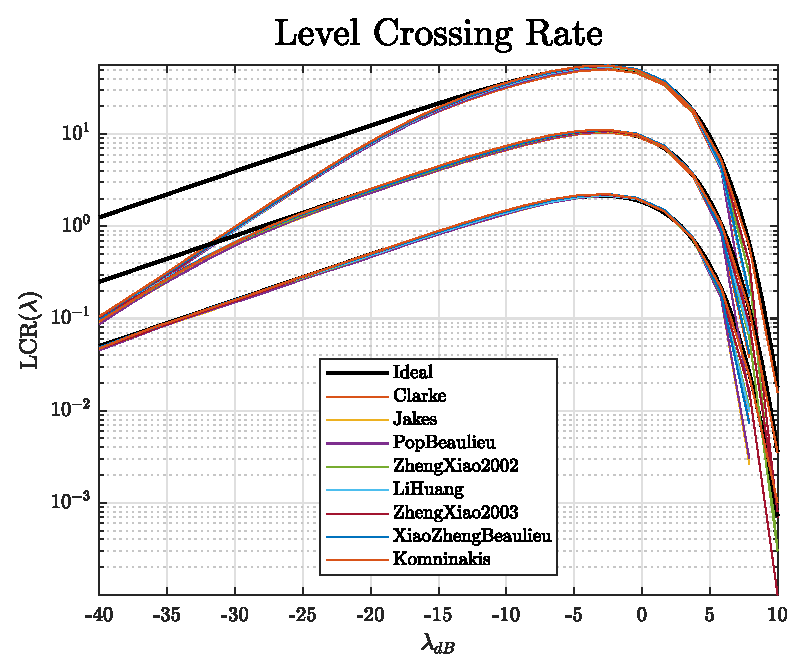
\includegraphics[width=\linewidth]{img/multiLCR.eps}
	\end{minipage}
	\hfill
	\begin{minipage}{.49\linewidth}
		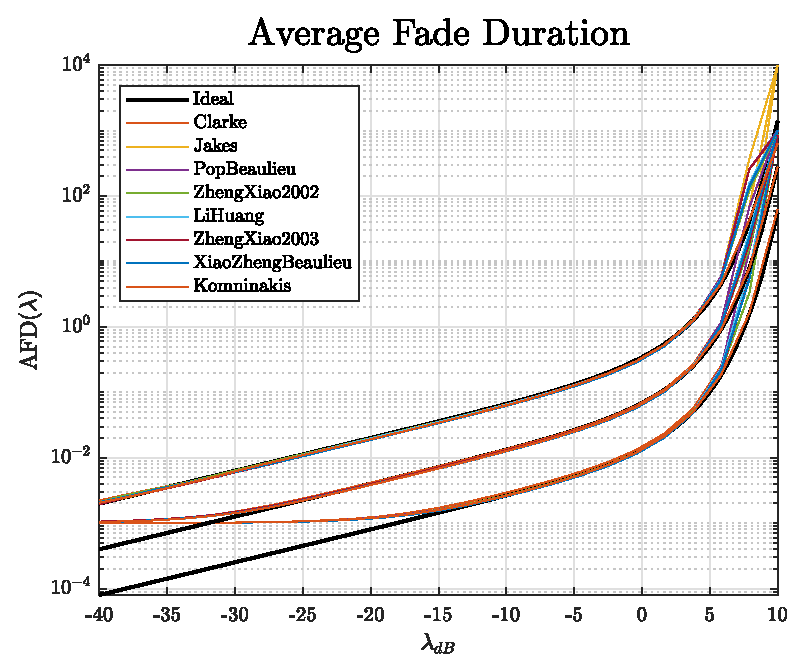
\includegraphics[width=\linewidth]{img/multiAFD.eps}
	\end{minipage}
	\hfill
	
	\caption{Plots for threshold-based statistics. The normalized thresholds are shown as  $\lambda_{dB} \triangleq 20\, \log_{10} \lambda$}
	\label{fig:LCR_AFD}
\end{figure}

The last statistics that I'm going to submit here were not present in all of the reference papers, but I think they are really important if not crucial (for example in channel coding design). A short explanation and ideal formulas were given in Sec.~\ref{subsec:math_models}, Eqs.~\ref{eq:LCR},\ref{eq:AFD}.

Starting from \textit{LCR}, it is possible to see from Fig.~\ref{fig:LCR_AFD} how different values for $f_dT$ ($0.05$, $0.01$ and $0.002$) yield very different results. In particular for low thresholds, the higher $f_dT$ the earlier the deviation from the ideal formula begins. This can be seen in exactly the same way for all of the proposed simulators, hence it's probably caused by something more fundamental. Reference \cite{A3} attributes this phenomenon to the fact that for fast fading (or low sampling rate, i.e. a high value of $f_dT$), some very narrow troughs cannot be correctly sampled, thus giving an underestimate of the level crossing rate. As the fading slows down (or sampling rate increases, i.e. $f_dT$ decreases) more and more fine troughs can be correctly sampled. This, of course, only postpones the problem, but if the critical threshold is low enough for your specific purpose, then the model can be used.
For high thresholds, instead, there are some major differences among the simulators: here \textit{Komninakis} is definitely the best one being almost identical to the ideal curve up to $10$ dB. \textit{ZhengXiao2003} and \textit{ZhengXiao2002} are respectively the second and third best ones, but usually reaching the $10$ dB threshold about an order of magnitude lower. All the other simulators do not even register any crossing above $8$ dB. From $5$ dB and below, instead, they all perform perfectly. Note that we are usually interested in low thresholds, since they are the ones responsible for errors, so the low precision towards higher levels may be considered of secondary importance.

Similar considerations can be done for the \textit{AFD}: an increasing $f_dT$ yields worse performance towards lower thresholds due to resolution problems: in this case, a constant sampling period $T=1 ms$ was chosen, varying the Doppler spread as for the \textit{LCR} test. Note that the fade duration obviously cannot go below $1ms$, and higher/lower values of $f_dT$ make this problem arise sooner/later. Once again, \textit{Komninakis} tend to perform almost perfectly while all the others overshoot even considerably the ideal statistics. But still, we are usually interested for how long the channel will return erroneous bits, meaning for how long it will stay below a (low) threshold. So, as for the \textit{LCR}, also for the \textit{AFD} high levels may be considered not important and, again, it should be checked whether the product $f_dT$ is suitable for the particular problem.

%%%%%%%%%%%%%%%%%%%%%%%%%%%%%%%%%%%%%%%%%%%%%%%%%%%%%%%%%%%%%%%%%%%%%%%%%%%%%%%%%%%%%%%%%%%%%%%
%%%%%%%%%%%% Simulation Time
%%%%%%%%%%%%%%%%%%%%%%%%%%%%%%%%%%%%%%%%%%%%%%%%%%%%%%%%%%%%%%%%%%%%%%%%%%%%%%%%%%%%%%%%%%%%%%%
\subsection{Performance Evaluation}

\begin{figure}
	\hfill
	\begin{subfigure}[t]{.49\linewidth}
		\centering
		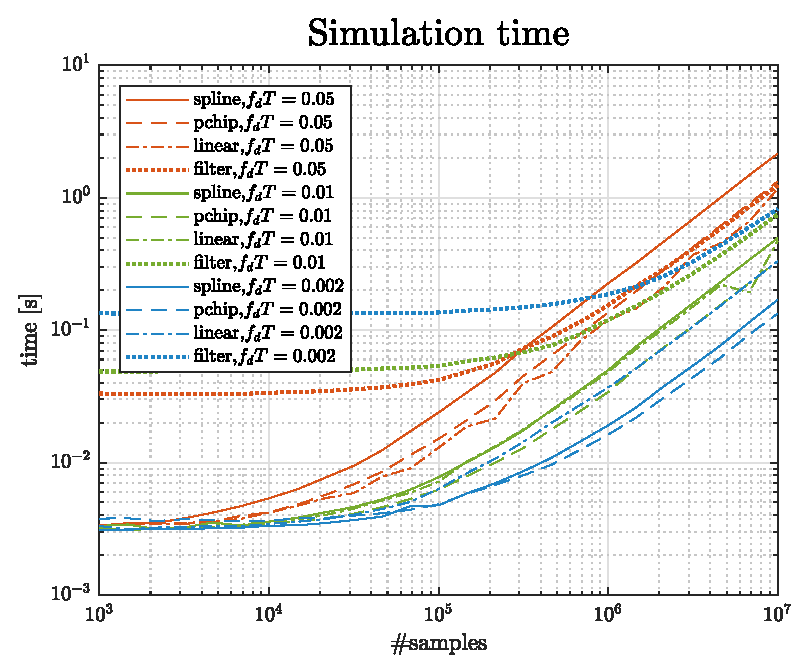
\includegraphics[width=\linewidth]{img/simTime_Komninakis.eps}
		\subcaption{Kominakis Simulation Time}
		\label{fig:KomninakisSimTime}
	\end{subfigure}
	\hfill
	\begin{subfigure}[t]{.49\linewidth}
		\centering
		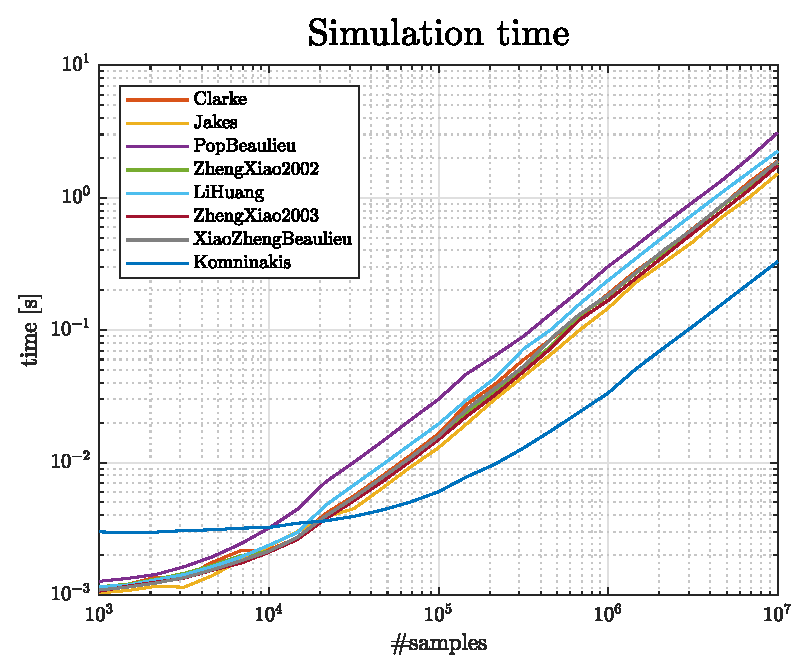
\includegraphics[width=\linewidth]{img/simTime.eps}
		\subcaption{Overall Simulation Time}
		\label{fig:overallSimTime}
	\end{subfigure}
	\hfill
	
	\caption{Simulation time for optimized implementations}
	\label{fig:simTime}
\end{figure}

\begin{wrapfigure}{R}{.45\linewidth}
	\centering
	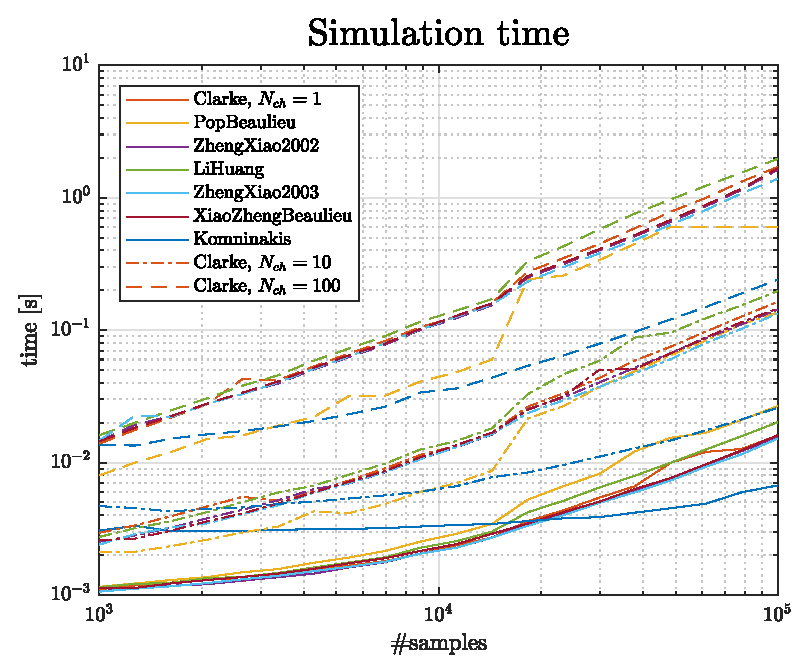
\includegraphics[width=\linewidth]{img/multiSimTime.eps}
	
	\caption{Simulation time with different number of channels}
	\label{fig:multiSimTime}
\end{wrapfigure}

One final test that i decided to do is a performance evaluation. This is quite delicate, though: a fine optimization should be carefully done for each one of the 8 simulators implemented in order to obtain meaningful results. Also, the results are machine and probably even CPU architecture dependent. In order to squeeze every last bit of performance, MATLAB's proprietary profiler has been exploited over and over to optimize at the best of my capabilities every simulator. For what concerns the architecture, MATLAB R2017a has been used, running over a 64-bit Windows 10 machine equipped with an Intel Core i5-2500K (overclocked @4.11 GHz) and 8 GB of RAM. Each test has been carefully designed in order to maximize the memory usage without exceeding it (which would have artificially hurt performance). Finally, timings were taken through MATLAB using the \texttt{tic-toc} instructions around a call to the function \texttt{createChannel}. Multiple simulations are then performed (at least 10) until the $95\%$ \textit{Confidence Interval} falls below a $10\%$ error from the mean.

For the first test, I had to decide which type of interpolation for \textit{Komninakis}' simulator and $f_dT$ product to use for all of the previous tests. Fig.~\ref{fig:KomninakisSimTime} shows how different values for $f_dT$ affect performance over a broad range of simulated samples. I want to recall that \textit{Komninakis'} filter is set to work at a fixed $f_dT=0.1$, hence for lower values of $f_dT$ a lower number of Complex Gaussian random variables will have to be created, a higher interpolation factor will be need and, thus, a narrower low-pass interpolation filter will have to be designed. This is perfectly reflected in the figure: for the filter interpolation, a much higher initial cost is needed in order to design the low-pass filter, and this cost raises the narrower the filter. For the polynomial interpolation, instead, no such cost is required thus yielding better performance when less random variables are needed (polynomial interpolation is low cost). Furthermore, the \textit{spline} interpolation, as expected, is the most expansive one, while \textit{pchip} is a bit more efficient. I expected \textit{linear} interpolation to be by far the most efficient one but apparently it is not so. In any case, statistics for this simple interpolation were quite bad, whereas \textit{spline} and \textit{pchip} were comparable. For the high initial cost, then, I didn't even considered the \textit{filter} method but it may be a possibility for a very high number of samples. For these reasons in the end I decided to use \textit{pchip} as the main interpolation method.

Looking, now, at Fig.~\ref{fig:overallSimTime}, the results for a single channel simulation, we clearly see two things at a glance: the \textit{Komninakis} simulator starts higher than the others but quickly surpasses them all, while they stay quite close to each other. The former is partially expected since higher overhead is required by all of the different steps of the simulator, while, apparently, \textit{pchip} interpolation is much faster than computing trigonometric functions, justifying the title of \cite{A3}. The latter is also quite expected, but maybe not this much close together. A few things to notice: \textit{Jakes'} simulator, fortunately, is the fastest one but \textit{PopBeaulieu} is by far the slowest one. Note also that \textit{Clarke}'s simulator doesn't perform so bad compared to the others.

One last curiosity that I had was about how simulators would behave with a higher number of independent channels. Due to the deterministic nature of \textit{Jakes'} simulator, I did not include it in this comparison since it would have simply made a repetition of the first channel. I was able, though, to keep the same colors for all the other simulators in order to have a better and unified visual presentation (Fig.~\ref{fig:multiSimTime}). The strangest result is certainly given by \textit{PopBeaulieu}: with only one channel it performs the worst while for 10 and 100 is actually the best one among the \textit{SOS} type of simulators, even with exceptional results up to $15 \cdot 10^3$ samples, then suddenly it aligns with the rest of the group. Here it can be fully appreciated the computational efficiency of \textit{Komninakis}' simulator: it can improve the simulation time up to a full order of magnitude!
\section{Conclusions} % max 1/2 page
% Obj. 1: Summariza what you did in the project
% Obj. 2: Lessons learned
\label{sec:conclusions}

In the end, 8 different Rayleigh channel simulators have been implemented and both their statistical and computational performance have been tested. Excluding \textit{Jakes'} and \textit{PopBeaulieu}'s simulators, all the others have very similar performance, and usually very close to the ideal case. Different simulators shined for particular reasons: while \textit{Komninakis} has outstanding performance for what concerns both computational complexity and fading statistics, it also has quite poor correlation statistics; on the other hand \textit{Clarke}'s original model actually yields very good performance all around without resulting as slow as it may have been thought. One thing to say, though, is that while for all the other \textit{SOS} simulators further optimization could (possibly) be done, it would be much more difficult for the latter since no symmetries whatsoever are present.

Thanks to this project I had the possibility to try out many new MATLAB's programming techniques that I recently learned from a few Mathwork's courses. Now my code performs better, is more robust, and also well commented, documented and organized. Furthermore, I now have many simulators ready to use if ever needed and a full performance characterization for all of them.


\nocite{*}
\printbibliography

\end{document}
